% --------------------------------------------------------------
% This is all preamble stuff that you don't have to worry about.
% Head down to where it says "Start here"
% --------------------------------------------------------------
 
\documentclass[12pt]{article}
\usepackage{graphicx}
\usepackage[margin=1in]{geometry} 
\usepackage{amsmath,amsthm,amssymb}
\usepackage{courier} % for inline code
%%% This sectino for coloring hyperlinks:
\usepackage{xcolor} % for hyperlinks
\usepackage[colorlinks = true,
            linkcolor = blue,
            urlcolor  = blue,
            citecolor = blue,
            anchorcolor = blue]{hyperref}
\newcommand{\MYhref}[3][blue]{\href{#2}{\color{#1}{#3}}}%

\usepackage{comment} % to comment out large sections
\usepackage{changepage}% for indenting stuff

%%% This section for header and footer settings
\usepackage{fancyhdr}
\pagestyle{fancy}
\lhead{}
\chead{}
\rhead{}
\lfoot{}
\rfoot{}
\cfoot{Vital $\vert$ NYU Tandon}
\renewcommand{\headrulewidth}{0pt}
\renewcommand{\footrulewidth}{1pt}



\newcommand{\N}{\mathbb{N}}
\newcommand{\Z}{\mathbb{Z}}
 
\newenvironment{theorem}[2][Theorem]{\begin{trivlist}
\item[\hskip \labelsep {\bfseries #1}\hskip \labelsep {\bfseries #2.}]}{\end{trivlist}}
\newenvironment{lemma}[2][Lemma]{\begin{trivlist}
\item[\hskip \labelsep {\bfseries #1}\hskip \labelsep {\bfseries #2.}]}{\end{trivlist}}
\newenvironment{exercise}[2][Exercise]{\begin{trivlist}
\item[\hskip \labelsep {\bfseries #1}\hskip \labelsep {\bfseries #2.}]}{\end{trivlist}}
\newenvironment{problem}[2][Problem]{\begin{trivlist}
\item[\hskip \labelsep {\bfseries #1}\hskip \labelsep {\bfseries #2.}]}{\end{trivlist}}
\newenvironment{question}[2][Question]{\begin{trivlist}
\item[\hskip \labelsep {\bfseries #1}\hskip \labelsep {\bfseries #2.}]}{\end{trivlist}}
\newenvironment{corollary}[2][Corollary]{\begin{trivlist}
\item[\hskip \labelsep {\bfseries #1}\hskip \labelsep {\bfseries #2.}]}{\end{trivlist}}
\date{} % don't show date
\usepackage{parskip}% http://ctan.org/pkg/parskip

\begin{document}
%\raggedright % comment this out for center justification

% --------------------------------------------------------------
%                         Start here
% --------------------------------------------------------------

\title{\huge{\textbf{Vital}}\\\large{User Guide}}%replace X with the appropriate number
\author{New York University\\ %replace with your name
Tandon School of Engineering} %if necessary, replace with your course title
 
\maketitle

\section*{What is Vital?}
Vital is a private cloud platform that provides students with hands-on learning experiences within a virtual lab environment. Courses at NYU Tandon make use of Vital by offering students the opportunity to experiment with their own virtual machines via lab-based assignments and projects.

This document serves as a general introductory guide for new Vital users. Contact information for issues and technical support is provided in the final section.


You can find the Vital homepage at: \MYhref{https://vital.engineering.nyu.edu/vital/login/}{https://vital.engineering.nyu.edu/vital/login/}

\section*{Account Creation}
First-time users are required to create a new account before they can access Vital. Click the `Signup for a new account’ link on the homepage.

{%
\centering
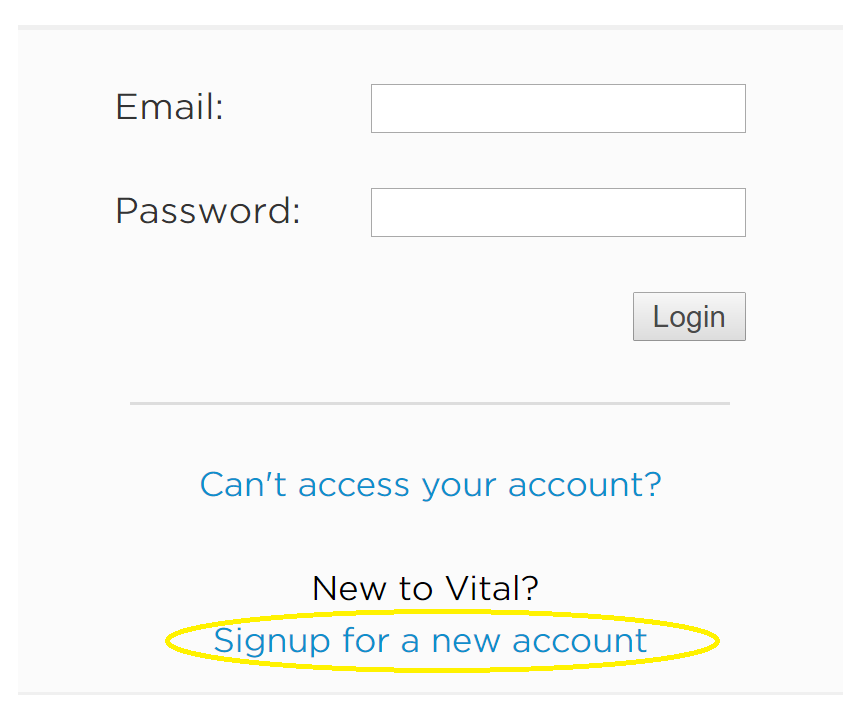
\includegraphics[scale=0.40]{account_creation.png}

}


Clicking on this link will redirect you to a page where you may submit your student information and complete the registration process. 

{%
\centering
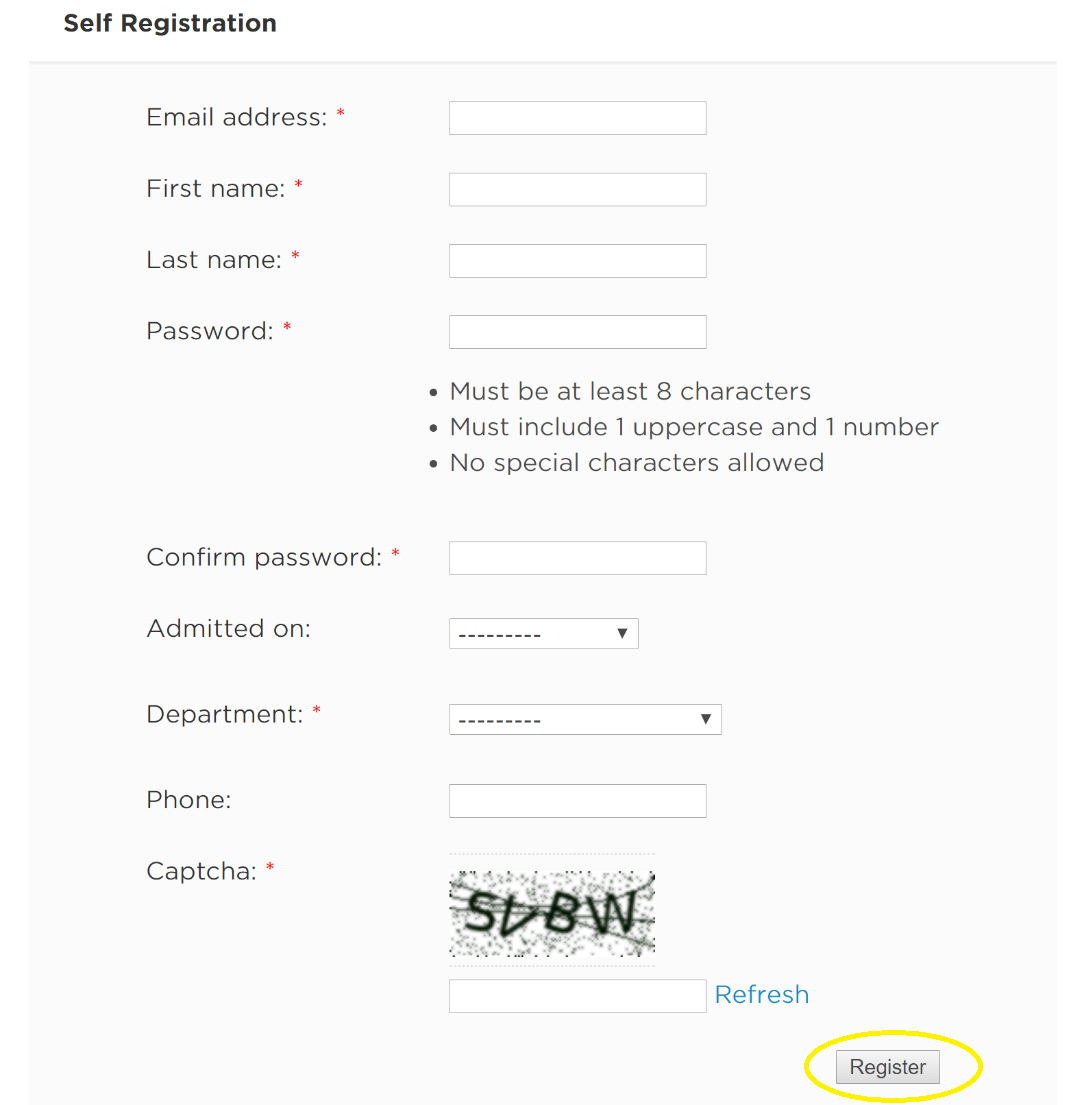
\includegraphics[scale=0.50]{self_registration.png}

}

When choosing a password, please be sure to meet the minimum complexity requirements. \textbf{We advise against reusing passwords that you have already registered for any other system}. Upon submitting this form, you will be redirected back to the login page where you may authenticate to Vital using your new login credentials.

\section*{Course Registration}
After you have created a Vital user account, you will need to supply a registration code in order to get access to your course-specific lab environment. This code will be provided to you by your instructor.

Upon authenticating to Vital, you will be presented a page which contains links to your course lab environments. This list will appear empty if this is your first time registering for a course. You may add a course by clicking the `Add course' link and providing your course registration code.

 
{%
\centering
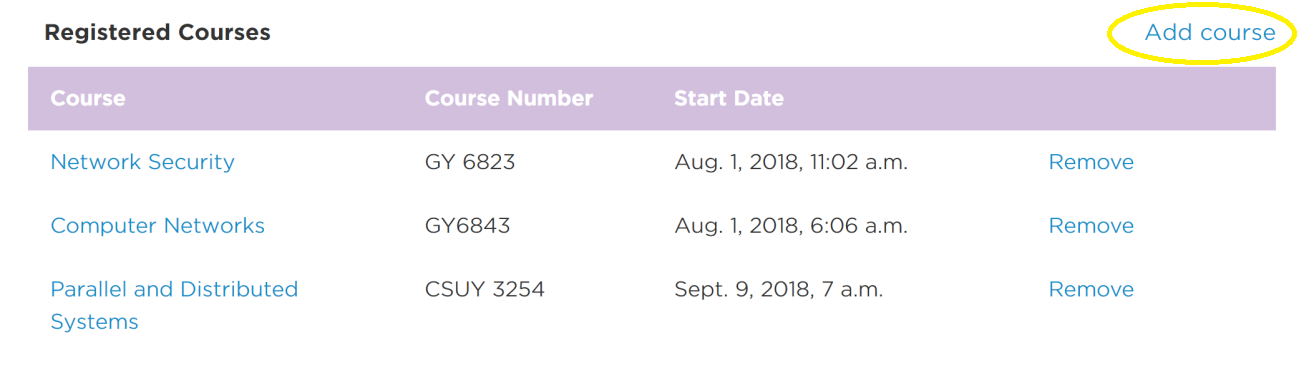
\includegraphics[width=\linewidth]{course_registration.png}

}

\section*{Vital Features}
Now we are ready to get hands-on with some of the infrastructure provided by Vital. In this section, we will examine the features of the platform and offer best practices. 

Vital infrastructure uses the same default login for each course environment:
\begin{adjustwidth}{2.5em}{0pt}
\textbf{username:} student\\
\textbf{password:} student
\end{adjustwidth}

\subsection*{Course Environment}
Each course within Vital is unique. Certain course networks enable access to the Internet while others may be private. The virtual machines found within each course environment are preconfigured with the applications you need to build and test your solutions.

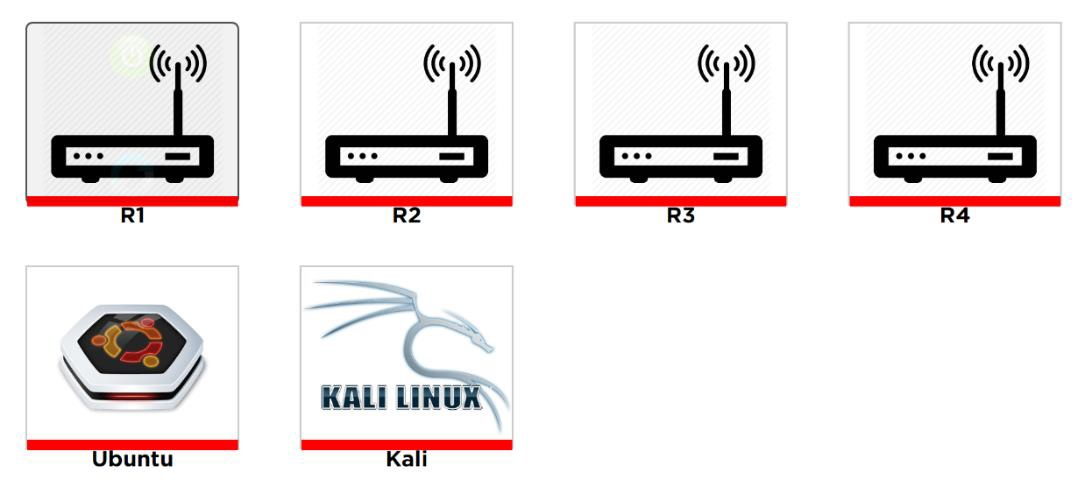
\includegraphics[scale=0.50]{course_environment}

As you can see in the image above, we are given access to six virtual machines in this particular course – Ubuntu, Kali Linux, and four routers. 

\subsection*{Starting \& Stopping Virtual Machines}
Virtual machines (VM) with an underlying red status bar are in an ``off” state. If you hover your mouse pointer over any of the machines found within this course page, a green power icon will appear. Clicking this icon will start the VM.

{%
\centering
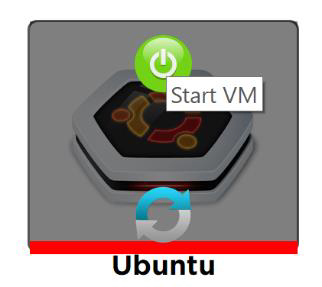
\includegraphics[scale=0.50]{start_vm.png}

}
After you have started the machine, the status bar will change to green to indicate that the VM is now running. The ‘View console’ icon will now appear as a new mouseover option. Clicking the ‘View console’ icon will launch the VM’s interface. 


{%
\centering
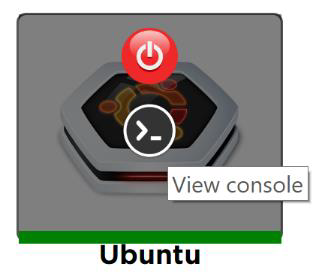
\includegraphics[scale=0.50]{view_console.png}

}
Notice that after starting the VM, the green power icon has changed to red. Clicking the red power icon will turn the machine off.

After clicking ‘View console’ and logging in using the default username and password, you will be presented the following interface (Ubuntu):

{%
\centering
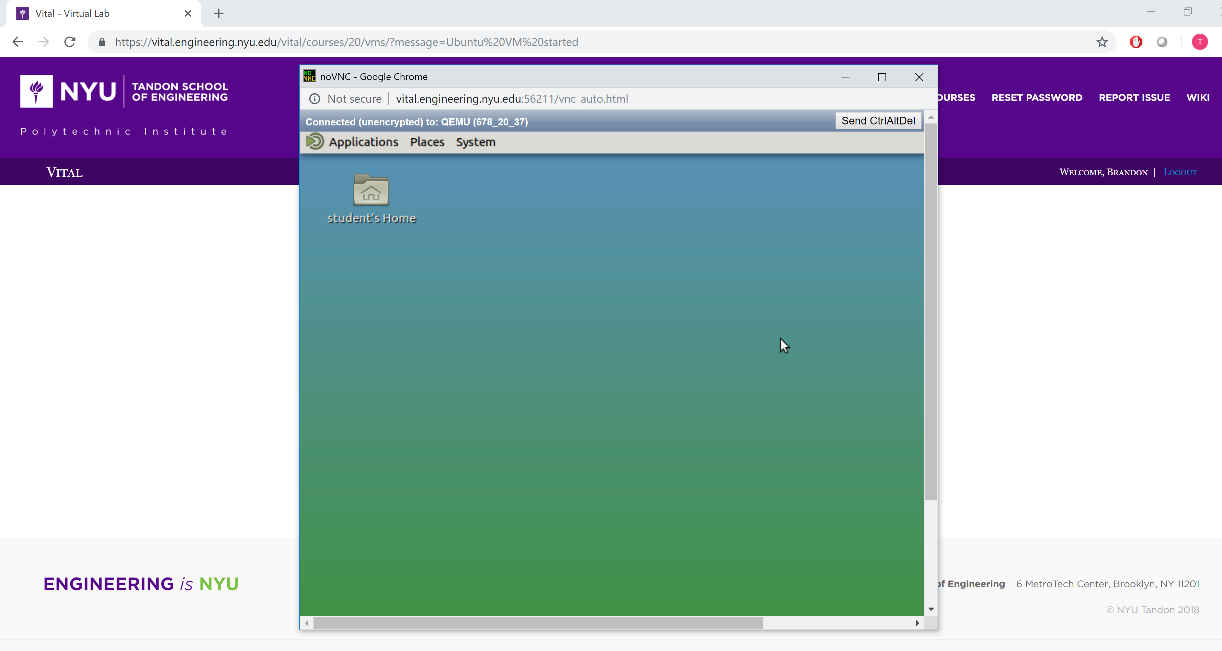
\includegraphics[scale=0.30]{vm_interface.png}

}

\textbf{Do not forget to shut down all machines and log off Vital after completing your lab session}. Clicking the ‘Logout’ link in the upper-right corner will automatically send the shutdown signal to all active machines. Leaving machines online for an extended period of time will result in a warning email.


\subsection*{Reimaging Virtual Machines}
While working on labs there may be situations in which you may need to restore a machine to its initial state. To accomplish this Vital gives students the option to reimage a virtual machine. \textbf{Please be aware that this process will completely erase all user-specific data on the machine and restore it to its initial default settings}. Data deleted in this way \textbf{cannot be recovered}. Make sure you have saved your work elsewhere before initiating this process.  You can reimage a machine by selecting the blue arrow mouseover option.


{%
\centering
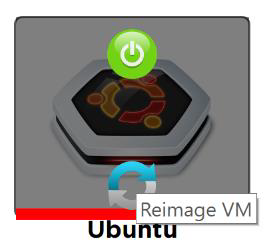
\includegraphics[scale=0.50]{reimage_vm.png}

}

\subsection*{SFTP File Transfers}
SSH File Transfer Protocol (SFTP) enables you to move files from one computer to another. You may need to do this for certain assignments. You must either be on the NYU network or connected to the NYU VPN to resolve the domain name of the SFTP server (sftp.engineering.nyu.edu / 128.238.77.36). If you are not presently on the NYU network, \MYhref{https://www.nyu.edu/life/information-technology/getting-started/network-and-connectivity/vpn.html}{click here} for information on how to setup a VPN connection to NYU.

Most operating systems come equipped with SFTP software which is accessible via the command line. You can authenticate to the SFTP server using your Vital username and password.

For example:
\begin{adjustwidth}{2.5em}{0pt}
\texttt{
> sftp <username>@128.238.77.36
}

\texttt{
> <password>
}
\end{adjustwidth}


After authenticating we can upload a file by executing:
\begin{adjustwidth}{2.5em}{0pt}
\texttt{
sftp> put <path to file>
}

\texttt{
sftp> exit
}
\end{adjustwidth}
{%
\centering
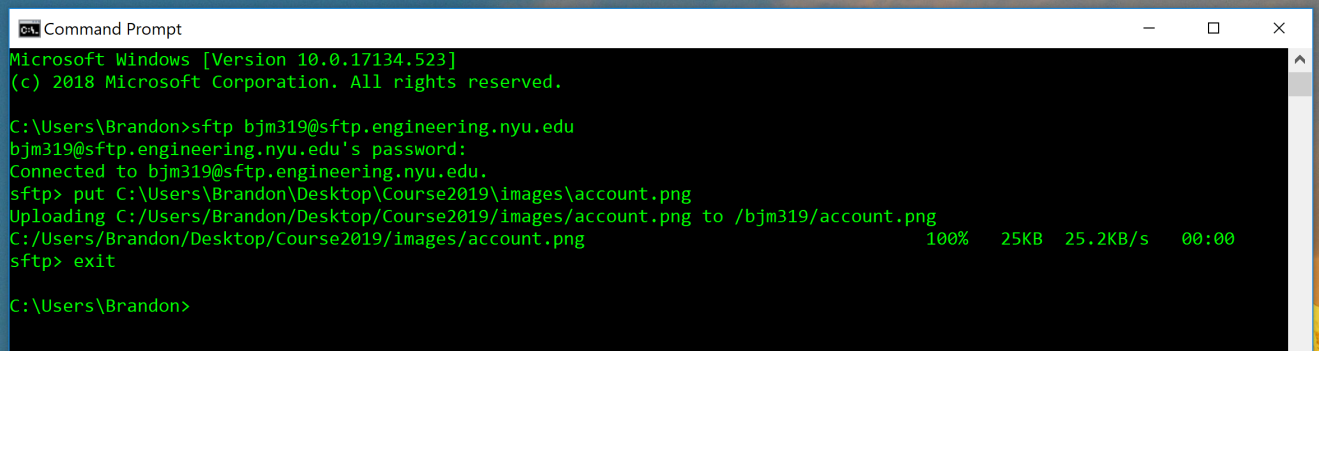
\includegraphics[width=\linewidth]{sftp1.png}

}


Once you have uploaded your files to the SFTP server, you can retrieve them from within the lab environment by executing the following commands:
\begin{adjustwidth}{2.5em}{0pt}
\texttt{
> sftp <username>@128.238.77.36
}

\texttt{
sftp> get <filename>
}

\texttt{
sftp> exit
}
\end{adjustwidth}
{%
\centering
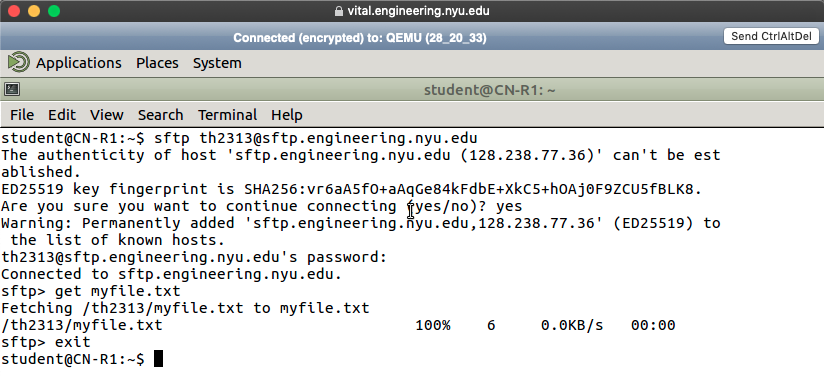
\includegraphics[width=\linewidth]{sftp2.png}

}

Once logged in to the SFTP server you can use the following command to see all options:
\begin{adjustwidth}{2.5em}{0pt}
\texttt{
sftp> ?
}
\end{adjustwidth}

% \newpage

\iffalse % comment out the entire VPN section for now
\section*{NYU VPN}
Download Cisco AnyConnect Client: \\
\MYhref{https://www.cisco.com/c/en/us/support/security/anyconnect-secure-mobility-client/tsd-products-support-series-home.html}{https://www.cisco.com/c/en/us/support/security/anyconnect-secure-mobility-client/tsd-products-support-series-home.html}

Connect to the VPN by supplying \textbf{vpn.nyu.edu} and using your two-factor authentication. 


{%
\centering
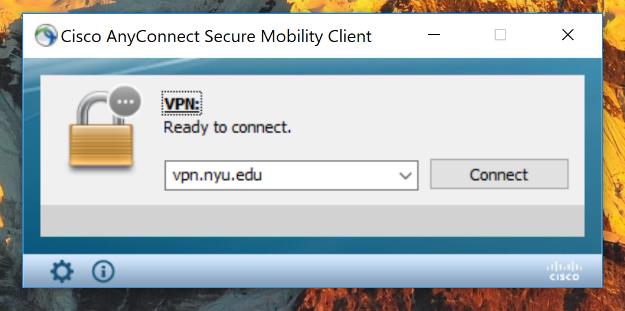
\includegraphics[scale=0.75]{vpn1.png}

}
After clicking ‘Connect’, you will be prompted to authenticate. In the example below, the first password is your NYU account password. The second password is your two-factor authentication code.

{%
\centering
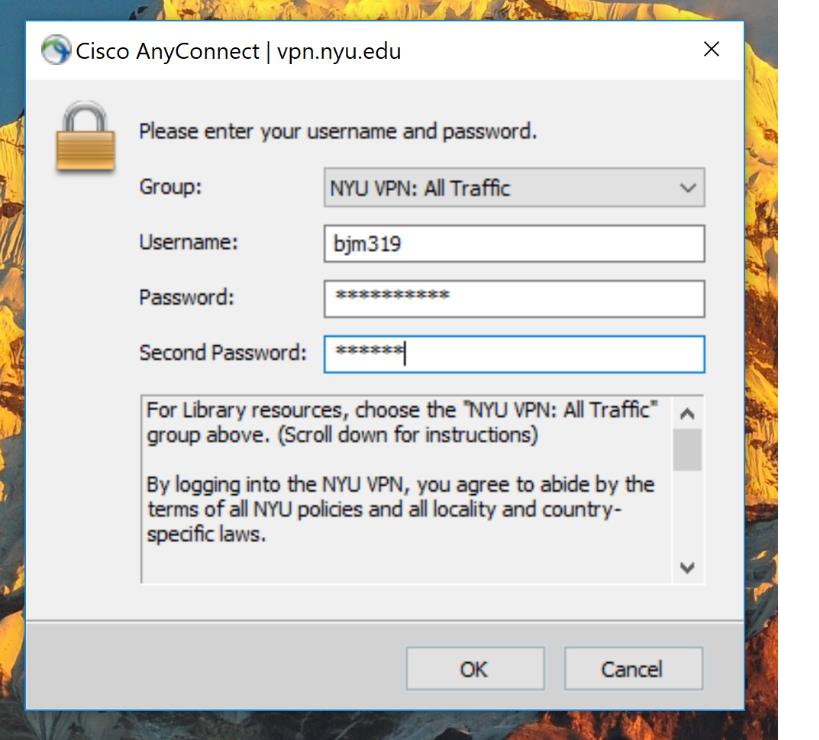
\includegraphics[scale=0.5]{vpn2.png}

}
\fi

\section*{Troubleshooting and Reporting Issues}
Please report any issues you may encounter while using Vital to our admin team at \\ \MYhref{mailto:vital@nyu.edu}{vital@nyu.edu}.

% --------------------------------------------------------------
%     You don't have to mess with anything below this line.
% --------------------------------------------------------------
 
\end{document}